% Indicate the main file. Must go at the beginning of the file.
% !TEX root = ../main.tex

%----------------------------------------------------------------------------------------
% CHAPTER TEMPLATE
%----------------------------------------------------------------------------------------


\chapter{Marc de treball i conceptes previs} % Main chapter title

\label{Marc de treball i conceptes previs} % Change X to a consecutive number; for referencing this chapter elsewhere, use \ref{ChapterX}

%----------------------------------------------------------------------------------------
% SECCIÓ 1: Marc de treball i conceptes previs
%----------------------------------------------------------------------------------------
Aquí s'expliquen tots els conceptes que cal saber per poder entendre tot el que s'ha desenvolupat al projecte, des de la modelització fins al disseny web i la connexió client-servidor.
\section{Problemes de satisfacció de restriccions}
Els problemes de satisfacció de restriccions en anglès CSP, es defineixen com a un conjunt de n variables \( X = \{X_1, X_2, \ldots, X_n\} \), un conjunt \( D = \{D_1, D_2, \ldots, D_n\} \) de dominis per cada variable i un conjunt \( R = \{R_1, R_2, \ldots, R_n\} \) de restriccions aplicades sobre les variables del conjunt X, aquestes restriccions són relacions k àries entre les variables   on l'objectiu és trobar una assignació sobre el conjunt de variables X fent ús del domini D de cada variable que satisfaci totes les restriccions del conjunt R. Les assignacions de valors a les variables s'anomena interpretació, aquesta interpretació no té per què satisfer les restriccions imposades sobre les variables del conjunt X, però la interpretació que si satisfà totes les restriccions s'anomena model. Tot seguit un exemple del famós problema send more money:\\

Suposem que tenim les variables \( X = \{S, E, N, D, M, O, R, Y\} \) on el domini de cada variable és \( D = \{[0 .. 9], \ldots, [0 .. 9]\} \) i el que volem és satisfer la restricció \( R_1 = \{1000S + 100E + 10N + D + 1000M + 100O + 10R + E = 10000M + 1000O + 100N + 10E + Y\} \) a més també volem que tots els valors que prenguin les variables siguin diferents entre ells \( R_2 = \{alldiff(S, E, N, D, M, O, R, Y)\}\).\\
Una possible interpretació podria ser \(S=0, E=1, N=2, D=3, M=4, O=5, R=6, Y=7\) l'avaluació d'aquesta assignació sobre les restriccions seria:\\
$$ R_1 = \{4684 = 45217\} $$
$$ R_2 = \{alldiff(0, 1, 2, 3, 4, 5, 6, 7)\}$$\\
Aquesta interpretació no és model, ja que la restricció $R_1$ no se satisfà.\\
Una interpretació que sí que és model és la següent:
$$ S=9, E=5, N=6, D=7, M=1, O=0, R=8, Y=2 $$\\
Ja que satisfà les dues restriccions:\\
$$ R_1 = \{10652 = 10652\} $$
$$ R_2 = \{alldiff(9, 5, 6, 7, 1, 0, 8, 2)\}$$

Amb aquest exemple es pot veure com aquest tipus de problemes no tenen un ``mètode'' per ser resolts sinó que requereixen prova i error fins que no es topa amb la solució. La complexitat d'aquest tipus de problemes s'estudia a branca de la complexitat computacional, tot seguit s'expliquen les idees bàsiques sobre aquest camp de la computació.

\section{Complexitat computacional}
Per poder definir les diferents complexitats computacionals dels problemes de CSP, cal introduir el concepte de màquina de Turing la qual serveix de base per establir que és computable i que no.

\subsection{Màquina de Turing}
La màquina de Turing, inventada per Alan Turing el 1936, és un model de còmput que descriu la màquina més simple capaç de poder executar qualsevol algorisme informàtic. La màquina treballa amb un alfabet finit i consta d'una cinta de longitud infinita dividida en cel·les, cada cel·la pot contenir qualsevol símbol de l'alfabet. La màquina també compta amb un capçal el qual apunta a la cel·la actual i és capaç de fer operacions de lectura i escriptura sobre la cel·la que apunta. A més la màquina compta amb un conjunt finit d'estats i una taula finita d'instruccions, en funció del símbol llegit i l'estat actual, s'escull una de les instruccions de la taula que poden ser, moure el capçal a la dreta o esquerra, esborrar o escriure un símbol a la cel·la actual o bé canviar d'estat.

\subsection{Classes de complexitat}
A la teoria de la computació hi ha moltes classes de complexitat, referents a l'espai en memòria necessari per resoldre un problema i el cost en temps requerit. Per aquest treball només s'explicaran les classes que fan referència al temps de còmput, ja que és el factor principal que afecta el problema de CSP.

\subsubsection{Classe P}
El conjunt de complexitat P conté tots aquells problemes que tenen un algorisme específic per ser resolts, on el cost en temps d'aquest algorisme augmenta polinomialment en funció del nombre de variables implicades al problema. Per exemple trobar el valor mínim en una llista de nombres té un cost lineal $O(n)$ que augmenta en funció de la longitud de la llista, l'ordenació dels nombres d'una llista és un altre problema de la classe P que pot ser resolt amb cost $O(n\log{}n)$ . També es diu que un problema és de complexitat P si una màquina de Turing determinista els pot resoldre en temps polinòmic.

\subsubsection{Classe NP i NP-complet} \label{np and np-completeness}
Els problemes de la classe NP (Nondeterminitic Polinomial Time), són aquells que poden ser resolts en temps polinòmic per una màquina de Turing no determinista, és a dir una màquina de Turing la qual de manera no determinista sap a quins estats ha de canviar per trobar la solució en temps polinòmic. L'exemple més conegut d'aquest tipus de problema tracta del problema de satisfacció (SAT) on donat un conjunt de variables booleanes i una CNF és volt trobar quina assignació fa que la CNF avaluï cert. A més SAT forma part de la classe NP-complet que implica que qualsevol problema NP pot ser reduït en temps polinòmic a SAT. Finalment, els problemes NP tenen la particularitat que una solució trobada pot ser verificada en temps polinòmic, per exemple per al problema SAT seria tan senzill com assegurar que cada clàusula avalua cert el qual tindria un cost lineal $O(n)$.

\subsubsection{NP-hard}
La classe NP-hard és de les més curioses, ja que la seva intersecció amb el conjunt NP forma el conjunt de la classe NP-complet, es poden reduir en temps polinòmic a NP-hard, però no tots els problemes NP-hard es poden reduir en temps polinòmic a problemes NP, a més, i molt important, els problemes NP-hard que no formen part del conjunt NP no es poden verificar en temps polinòmic per una màquina de Turing determinista. Per exemple alguns problemes d'optimització són NP-hard, ja que donada una solució comprovar que sigui l'òptima requereix saber totes les solucions per determinar si la solució trobada efectivament és l'òptima.\\
Totes aquestes definicions són certes sota l'assumpció que \(P\neq NP\) i fins que es pugui demostrar el contrari les classes de complexitat continuaran sent així. En cas que es pogués demostrar \(P = NP\), qüestió que tracta d'un dels set problemes del mil·lenni la representació de les classes de complexitat tenint en compte els dos escenaris pot ser vista a la figura \ref{fig:time-complexity-sets}.

\begin{figure}
    \centering
    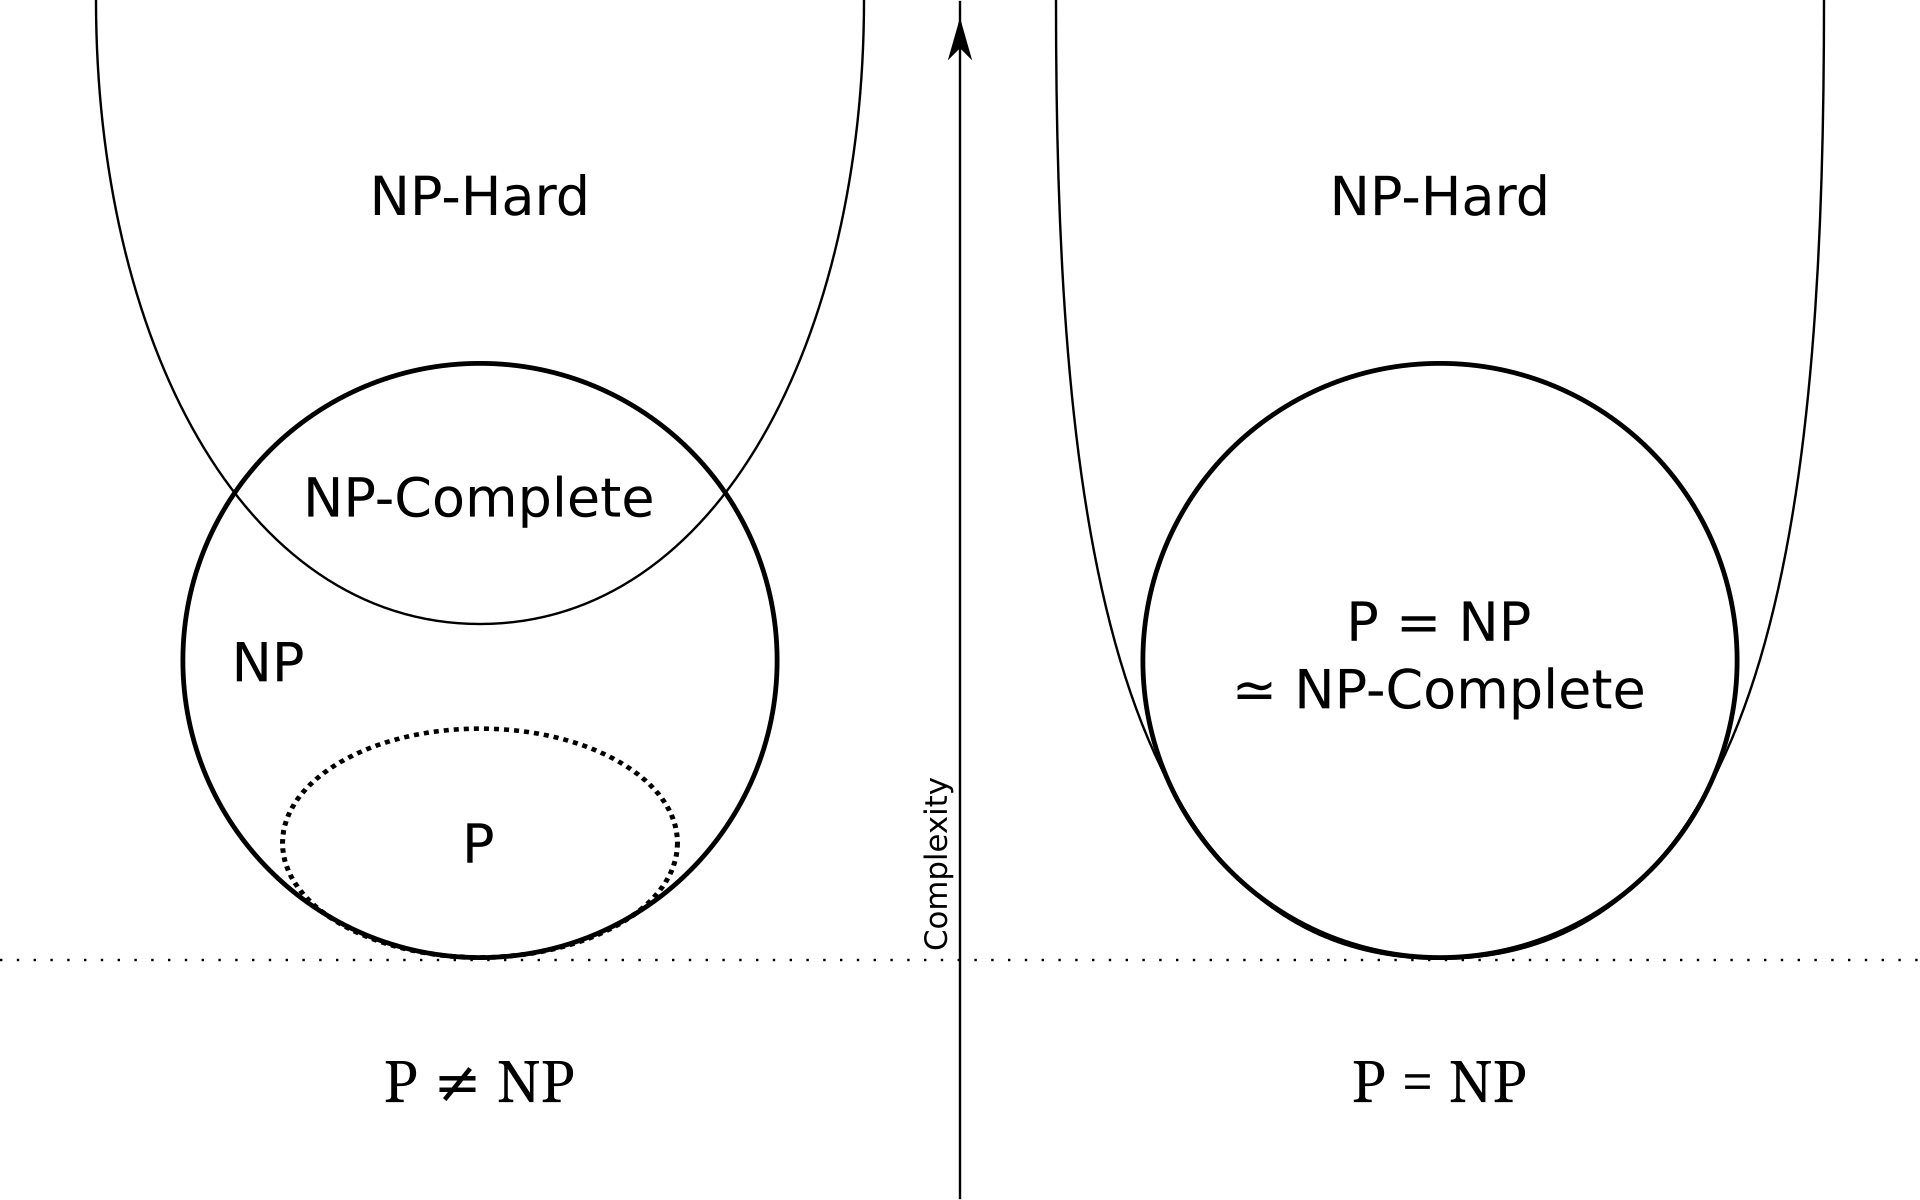
\includegraphics[width=1\linewidth]{Figures//miscelaneous/time-complexity-classes.png}
    \caption{Comparació de classes de complexitat si \(P\neq NP\) i \(P = NP\)}
    \label{fig:time-complexity-sets}
\end{figure}

\section{SAT}
Com s'ha explicat a la secció \ref{np and np-completeness}, SAT es troba dins el conjunt NP-complet, aquesta característica sumada a la simplicitat del problema, ha causat que sigui usat com a base per solucionar problemes del conjunt NP a causa de la propietat que tot problema del conjunt NP pot ser reduït a NP-complet. La tecnologia usada tracta dels SAT solvers els quals usen tècniques molt avançades per reduir el màxim el cost de la cerca per força bruta implícita als problemes d'aquesta complexitat.\\
Exemple del problema SAT.
Suposem que tenim la següent forma normal conjuntiva (CNF):\\
$$(a \lor b \lor c) \land (\lnot c \lor \lnot b) \land (\lnot a \lor \lnot b) \land (\lnot a \lor \lnot c) $$\\
Una interpretació possible seria:\\
$$ [a = cert, b = false, c = false]$$
$$(cert \lor false \lor false) \land (\lnot false \lor \lnot false) \land (\lnot cert \lor \lnot false) \land (\lnot cert \lor \lnot false) $$
$$cert  \land (cert \lor cert) \land (fals \lor cert) \land (fals \lor cert) $$
$$cert \land cert  \land cert \land cert $$
$$\textbf{cert}$$\\
Aquesta satisfà la fórmula, és model. A més aquesta CNF té la propietat que les assignacions que satisfan la fórmula són aquelles on només un literal és cert.\\

\begin{tabular}{ccc|c}
$a$ & $b$ & $c$ & $(a \lor b \lor c) \land (\lnot a \lor \lnot b) \land (\lnot a \lor \lnot c) \land (\lnot b \lor \lnot c)$ \\
\hline
1 & 1 & 1 & 0 \\
1 & 1 & 0 & 0 \\
1 & 0 & 1 & 0 \\
1 & 0 & 0 & 1 \\
0 & 1 & 1 & 0 \\
0 & 1 & 0 & 1 \\
0 & 0 & 1 & 1 \\
0 & 0 & 0 & 0 \\
\end{tabular}

Un dels problemes de SAT és que com que tracta de la satisfacció de les clàusules d'una CNF les quals estan formades per literals que són variables booleanes, hi ha problemes sobretot si aquests tracten amb variables numèriques que són molt difícils de reduir a SAT i encara que siguin reduïbles en certs casos generen tantes clàusules que usar un SAT solver passa a ser una opció inviable. Hi ha diverses alternatives que permeten fer modelitzacions similars a les que es farien amb SAT, però amb l'opció de poder usar variables de diferents tipus, per aquest projecte s'ha usat SMT (SAT Modulo Theories).

\section{SMT}
SMT o SAT Modulo Theories, tracta del problema de determinar si una fórmula matemàtica és satisfacible. A diferència del problema SAT, SMT incorpora múltiples teories, des d'aritmètica lineal fins a comparacions lògiques entre funcions no interpretades. Aquestes teories permeten l'ús de diferents tipus de dades (enters, reals, strings, llistes, arrays de bits...). A més també permet crear fórmules lògiques igual que a SAT però amb l'ús de les teories.\\
\begin{figure}
    \centering
    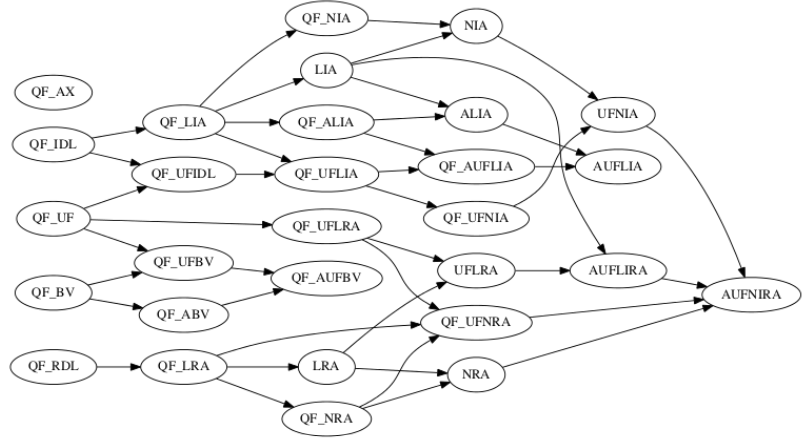
\includegraphics[width=0.5\linewidth]{Figures//miscelaneous/smt-lib-theories.png}
    \caption{Teories suportades per SMT-lib \cite{SMT-solving}}
    \label{fig:smt-theories}
\end{figure}

Els SAT solvers tenen un nucli que està especialitzat a trobar les assignacions satisfacibles de la fórmula fent ús de tècniques com CDCL. SMT aprofita aquest nucli i en fa una abstracció incorporant l'ús de les teories, tot seguit un exemple per entendre millor l'abstracció.
Suposem que tenim la següent fórmula:

$$ (c \le 5) \land (a \geq 3) \land (5a+b=c-3) $$
El primer pas és identificar cada teoria present a la fórmula i abstreure'n una variable booleana perquè el nucli SAT pugui resoldre.\\
$$ [A=(c \le 5), B=(a \geq 3), C=(5a+b=c-3)] $$
$$ A \land B \land C $$

Dins de les teories que la llibreria de SMT-lib suporta \ref{fig:smt-theories}, les variables A i B tracten de la teoria (integer rational difference logic o QF\_IDL) i la variable C la teoria (real/integer linear arithmetic). Amb l'abstracció feta i les teories identificades el solver primer resol la part SAT de la fórmula, si es troba una assignació vàlida es criden els nuclis que resolen les teories, en cas que hi hagi una assignació que satisfaci les variables abstretes la fórmula és satisfacible, en cas contrari, el nucli del SAT solver aprèn com a lema que la variable no pot ser assignada un valor positiu i continua fent solving fins que es demostra satisfacibilitat o no hi ha més assignacions disponibles.\\
En aquest exemple com la fórmula és molt simple el SAT solver demana als nuclis de les teories esmentades que avaluïn cert i aquestes per exemple podrien respondre el següent:\\
\(A \Rightarrow c=4 \Rightarrow 4\le5 \Rightarrow cert\)\\
\(B \Rightarrow a=3 \Rightarrow 3\geq5 \Rightarrow cert\)\\
\(C \Rightarrow b=-14 \Rightarrow (15-14=4-3) \Rightarrow cert\)\\
L'esquema de la figura \ref{fig:smt-solver-lazy} representa el procés de solving d'un SMT solver usant lazy solving.
\begin{figure}
    \centering
    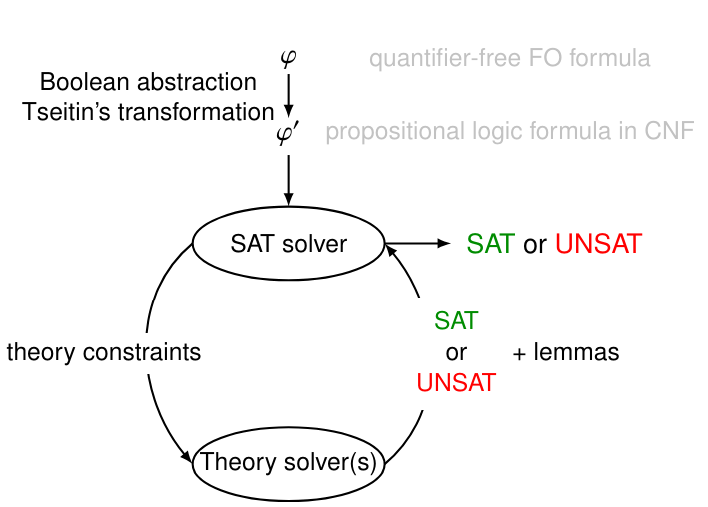
\includegraphics[width=0.5\linewidth]{Figures//miscelaneous/smt-lazy-zolver.png}
    \caption{Esquema d'un SMT solver lazy \cite{SMT-solving}}
    \label{fig:smt-solver-lazy}
\end{figure}

\section{Elements bàsics del joc Factorio}
Com s'ha explicat prèviament, Factorio és un joc d'automatització i ampliació de fàbriques en un món 2D basat en una graella. Els elements que el joc posa a disposició del jugador en són molts, així i tot, els bàsics per poder construir i automatitzar la producció d'objectes en són tres: inseridors, cintes transportadores i assembladors tot seguit una explicació en detall del comportament de cadascun.

\subsection{Cinta transportadora}
Les cintes transportadores o \textit{conveyor belts} serveixen per transportar elements d'un punt a un altre. Aquestes ocupen 1x1 caselles a la graella del món i poden prendre qualsevol de les 4 direccions cardinals. Transporten objectes de la casella actual a la següent casella apuntada per la cinta. Aquestes poden rebre objectes per qualsevol de les tres caselles adjacents diferents de la casella de sortida (la que apunta la cinta).
Al joc les cintes consten de dues pistes cadascuna amb la mateixa capacitat de transport d'objectes, però no s'ha tingut en compte aquesta mecànica, ja que de la manera que funciona afegeix molta complexitat.
La capacitat de transport d'una cinta, tenint només en compte una de les pistes, és de 450 objectes per minut.
\begin{figure}[ht]
    \centering
    \begin{subfigure}{0.45\textwidth}
        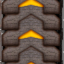
\includegraphics[width=\textwidth]{Figures/captures_joc/conveyor.png}
        \caption{Cinta transportadora a la graella del joc}
    \end{subfigure}
    \hfill
    \begin{subfigure}{0.45\textwidth}
        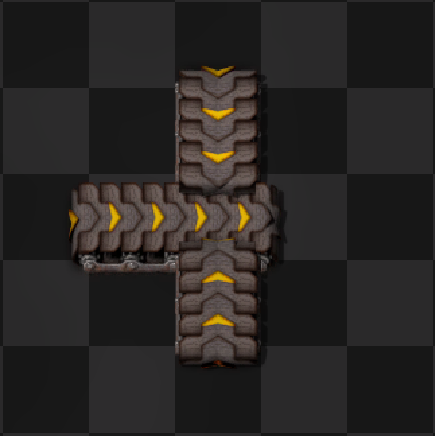
\includegraphics[width=\textwidth]{Figures/captures_joc/conveyor_inputs.png}
        \caption{Entrades permeses a una cinta transportadora}
    \end{subfigure}
    \caption{Cinta transportadora dins el joc i les seves possibles entrades}
    \label{fig:conveyor_in_out}
\end{figure}

\subsection{Inseridor}
Els inseridors o \textit{inserters} són braços robòtics que ocupen 1x1 caselles a la graella del món, permeten inserir i treure elements de cintes i assembladors.\\
Aquests poden treure elements de cintes que apuntin en qualsevol direcció i inserir objectes a cintes que no apuntin cap a ell. L'inseridor és l'únic element que pot suplir d'objectes a un assemblador i té el hàndicap que la seva capacitat de transport és de 50 objectes per minut.

\begin{figure}[H]
    \centering
    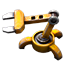
\includegraphics[width=0.33\linewidth]{Figures/captures_joc/inserter.png}
    \caption{Inseridor a la graella del joc}
    \label{fig:in_game_inserter}
\end{figure}


\begin{figure}[h]
    \centering
    \begin{subfigure}{0.45\textwidth}
        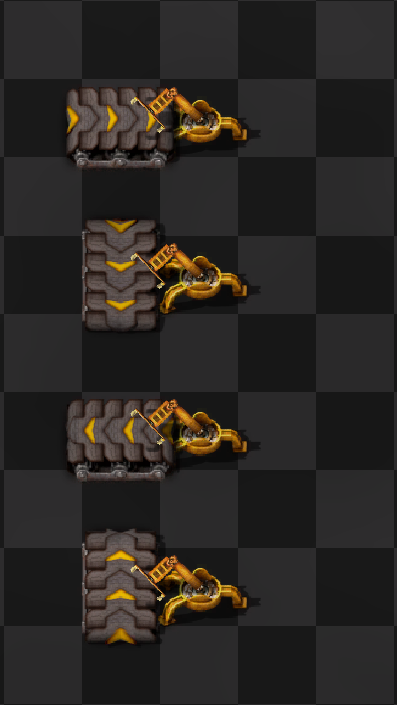
\includegraphics[width=\textwidth]{Figures/captures_joc/inserter_allowed_inputs.png}
        \caption{Entrades permeses}
    \end{subfigure}
    \hfill
    \begin{subfigure}{0.45\textwidth}
        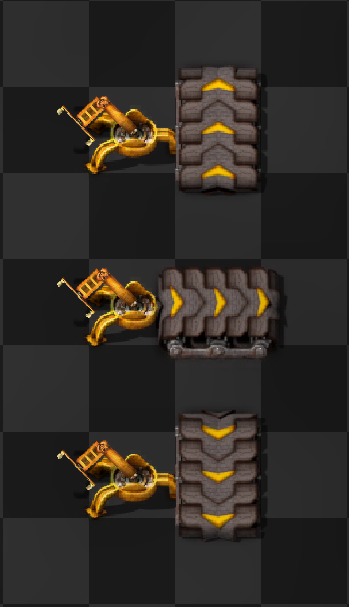
\includegraphics[width=\textwidth]{Figures/captures_joc/inserter_allowed_outputs.png}
        \caption{Sortides permeses}
    \end{subfigure}
    \caption{Orientacions de les cintes d'on un inseridor pot treure i agafar objectes}
    \label{fig:inserter_in_out}
\end{figure}

\subsection{Assemblador}
Els assembladors o \textit{assemblers} ocupen un espai de 3x3 caselles a la graella del món, aquests només poden rebre i treure objectes a través d'inseridors que estiguin en el mateix eix que qualsevol de les 12 caselles adjacents a l'assemblador.\\
La funcionalitat dels assembladors és convertir els materials d'entrada en objectes refinats, això es fa mitjançant receptes.

\begin{figure}[h]
    \centering
    \begin{subfigure}{0.45\textwidth}
        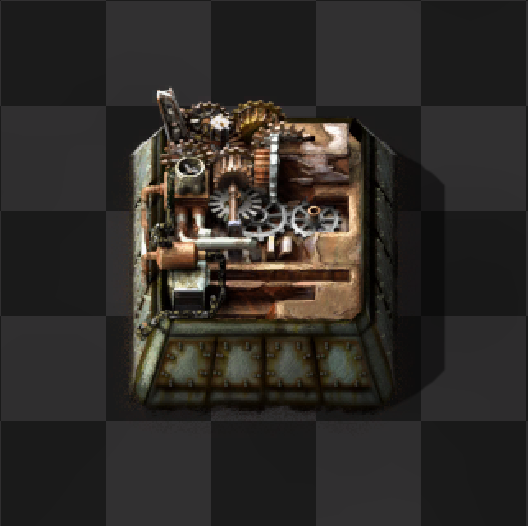
\includegraphics[width=\textwidth]{Figures/captures_joc/assembler.png}
        \caption{Assemblador a la graella del joc}
    \end{subfigure}
    \hfill
    \begin{subfigure}{0.45\textwidth}
        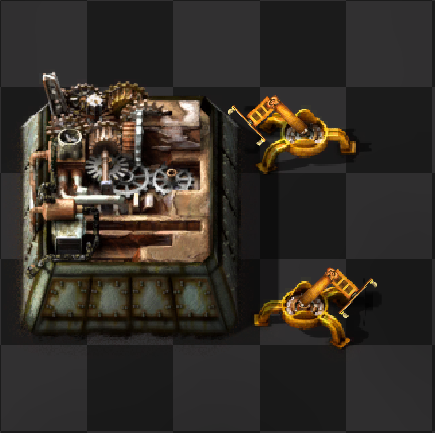
\includegraphics[width=\textwidth]{Figures/captures_joc/inserters_assembler.png}
        \caption{Inseridors interactuant amb l'assemblador}
    \end{subfigure}
    \caption{Representació de l'assemblador dins el joc}
\end{figure}

\subsubsection{Receptes} \label{subsec:recipes}
Les receptes només poden estar associades als assembladors, aquestes indiquen quins i quants objectes són necessaris per a la fabricació d'un altre objecte en un temps determinat.\\
Amb el temps que tarda un assemblador a produir els objectes d'una recepta i la quantitat d'objectes que requereix, podem calcular el nombre d'objectes per minut d'entrada i sortida màximes d'una recepta. Això ens serà molt útil més endavant per modelar receptes i el flux d'objectes.\\
En cas que un assemblador rebi més objectes per minut dels requerits per la recepta, aquests s'acumularan als inseridors i cintes que transporten l'objecte a l'assemblador, d'altra banda, si l'assemblador rep menys objectes per minut del que la recepta requereix, l'assemblador haurà d'esperar a tenir els objectes per iniciar la recepta fent que velocitat dels objectes fabricats es redueixi.\\
Totes les receptes que es produeixen a l'assemblador sempre generen un sol tipus d'objecte de sortida.

\begin{figure}[H]
    \centering
    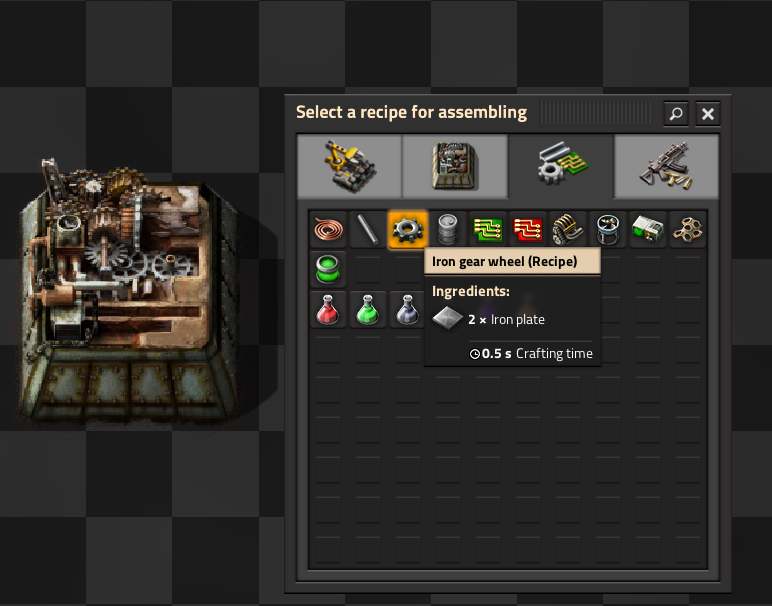
\includegraphics[width=0.5\linewidth]{Figures/captures_joc/assembler_recipe.png}
    \caption{Informació de la recepta d'un assemblador}
    \label{fig:assembler_recipe}
\end{figure}

\section{Conceptes relacionats amb els elements bàsics del joc}
Amb elements bàsics que poden constituir un \textit{blueprint} ja explicats, queda definir com aquests elements han d'interactuar entre ells per formar una fàbrica que respecti les mecàniques del joc, així doncs tot seguit s'explica com s'han dividit les interaccions entre elements, objectes que és es produeixen a la fàbrica...

\subsection{Ruta}
Una de les parts més importants del model és definir com la concatenació d'inseridors i cintes transportadores conformen una ruta. Perquè una ruta sigui vàlida no pot crear cicles, és a dir que una cinta o inseridor no pot entrar objectes a una cinta la qual era anterior a ella mateixa. També s'ha de tenir en compte l'orientació dels inseridors i cintes per complir amb les entrades i sortides vàlides anteriorment descrites. Una ruta també es pot bifurcar i unir.\\
Els inicis de ruta poden ser les caselles marcades com a entrada o bé la sortida d'un objecte d'un assemblador. D'altra banda, els finals de ruta poden ser les caselles marcades com a sortida o bé l'inseridor que afegeix elements a un assemblador.

\subsection{Tipus d'objectes}
Les cintes i inseridors han de poder dur objectes per les rutes que conformen, aquí entra la noció del tipus d'objectes, que depenen dels d'objectes especificats a les caselles d'entrada i sortida del \textit{blueprint}, juntament amb els objectes que un assemblador genera en funció de la recepta que tingui associada. Cal assegurar que a les 12 caselles adjacents a un assemblador les quals tenen inseridors entrant o sortint, no duguin o treguin objectes que la recepta associada a l'assemblador demana, també cal assegurar que una casella que forma part d'una ruta només pot dur un tipus d'objecte i finalment cal assegurar la correcta propagació dels objectes per les rutes.

\subsection{Quantitat d'objectes}
A banda de portar objectes, les rutes poden estar més o menys carregades, és a dir que cal alguna manera de saber quants objectes per minut porta una cinta o inseridor per poder saber quants objectes per minut ha de produir la recepta associada a un assemblador.\\
La recepta associada a un assemblador, com bé ha quedat explicat anteriorment, requereix un cert nombre d'objectes per minut per produir-ne uns altres a una densitat específica. Un dels problemes principals és que un assemblador pot rebre objectes requerits per la recepta en diferents quantitats que poden ser superiors o inferiors a la ràtio que marca la recepta, però els objectes que entrin en major quantitat no ho podran fer durant gaire temps, ja que ràpidament l'assemblador se saturarà d'objectes fent que la quantitat d'entrada s'anivelli a la quantitat respectiva de l'objecte que crea el coll d'ampolla.\\
Determinar correctament la quantitat d'objectes que hi ha a cada casella del \textit{blueprint} és una de les parts més crucials del problema, ja que és la que ens permetrà saber quants elements s'estan produint, cosa que volem maximitzar.

\section{El problema del blueprint} \label{sec:blueprint_problem}
El problema que es vol resoldre s'anomena el problema del \textit{blueprint}, el qual donades les entrades i sortides dels objectes, l'objecte que es vol produir i l'espai del qual es disposa, s'ha de maximitzar la quantitat produïda de l'objecte de sortida.\\
Per entendre millor apartats futurs on es parla d'implementacions concretes, es presenta un exemple, el qual tracta d'una instància resolta pel model. Amb aquest exemple es posa en context el problema i s'explica perquè aquest no és gens senzill.

\subsection{Exemple del problema}
Els inputs d'aquesta instància són les següents:\\
\begin{itemize}
    \item Mida: 8x8
    \item Entrades: (0,0) ``quadrat gris'' Xapes de ferro, (0,7) ``quadrat vermell'' Xapes de coure, (7,0) ``quadrat blanc'' Barres de plàstic
    \item Sortides: (7,7) ``cercle taronja'' Circuits avançats
    \item Objecte a produir: Circuits avançats
\end{itemize}

\begin{figure}
    \centering
    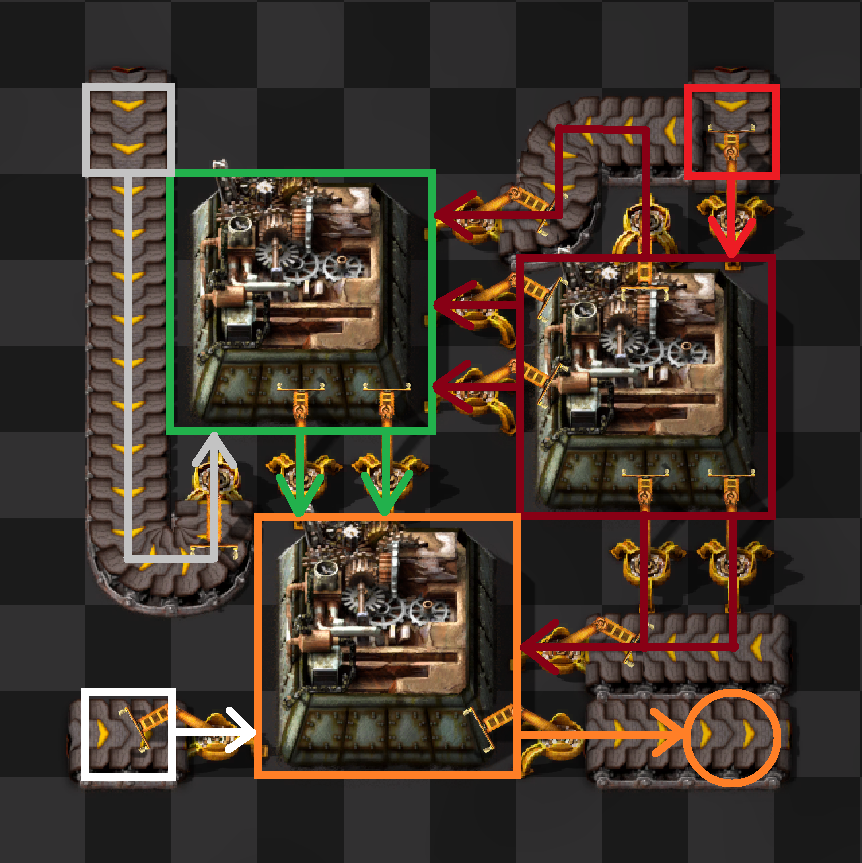
\includegraphics[width=0.75\linewidth]{Figures//captures_joc//exemples_model/exemple_base.png}
    \caption{Exemple base}
    \label{fig:solucio_exemple}
\end{figure}

Com es pot veure a l'exemple resolt \ref{fig:solucio_exemple}, per produït Circuits avançats s'han necessitat tres assembladors, un per cada recepta implicada en la producció de Circuits avançats, concretament es requereixen les receptes:
\begin{itemize}
    \item Cable de coure "assemblador emmarcat en carmí"
    \item Circuits electrònics "assemblador emmarcat en verd"
    \item Circuits avançats "assemblador emmarcat en taronja"
\end{itemize}


Com l'espai del \textit{blueprint} és molt ajustat hi ha rutes que només tracten d'un inseridor que agafa els objectes produïts d'un assemblador i els insereix directament al assemblador adjacent.\\

Pel que fa a la distribució dels objectes primer cal saber la quantitat d'objectes per minut que requereix i produeix cada recepta.\\
\begin{table}
\begin{tabular}{|c|c|c|}
\hline
\textbf{Recepta} & \textbf{Requereix} & \textbf{Produeix} \\ \hline

Circuit avançat & 
\begin{tabular}{@{}c@{}}
40 Cable de coure \\ \hline
20 Circuits electrònics \\ \hline
20 Barres de plàstic
\end{tabular} &  
10 Circuits avançats
\\ \hline

Circuit electrònic &
\begin{tabular}{@{}c@{}}
360 Cable de coure \\ \hline
120 Plaques de ferro \\ \hline
20 Barres de plàstic
\end{tabular} &
120 Circuits electrònics \\ \hline

Cable de coure & 120 Plaques de coure & 240 Cables de coure \\ \hline
\end{tabular}\\
\caption{Materials requerits i produïts per cada recepta}
\label{table:objectes_requerits}
\end{table}
Pel que fa als materials en cru que entren per les caselles emmarcades a la imatge, estan entrant les següents quantitats:

\begin{tabular}{|c|c|}
\hline
\textbf{Material} & \textbf{Quantitat d'entrada} \\ \hline
Placa de coure & 50\\ \hline
Placa de ferro & 98.06\\ \hline
Barra de plàstic & 20.0138\\ \hline
\end{tabular}\\

D'aquestes quantitats d'entrada no s'aprofiten tots els objectes pel fet que alguns assembladors no tenen prou inseridors de sortida per poder aprofitar tot el material. Aquesta ``pèrdua'' es tradueix en material que s'acumula a les cintes d'on els inseridors agafen els materials d'entrada pel assembladors, concretament la cinta a la posició (7,0) acumula 0.138 barres de plàstic, fent que la quantitat d'entrada de l'assemblador de circuits avançats sigui de 20 barres de plàstic per minut. D'altra banda, la cinta a la posició (5,1) acumula 78.06 plaques de ferro, fent que l'entrada a l'assemblador sigui de 20 plaques de ferro per minut. Finalment, les plaques de coure que entren per la casella (0,7) s'aprofiten totes.\\

Ara que ja s'han explicat les quantitats d'entrada i els materials que cada recepta requereix, es pot veure com l'assemblador carmí per poder processar les 50 plaques de coure per minut ha de poder extreure 100 cables de coure això ho fa mitjançant 5 inseridors, els quals es divideixen la quantitat de sortida en parts proporcionals fent que $3/5$ parts, és a dir 60 cables, es destinin a la producció de circuits electrònics i $2/5$ parts, és a dir 40 cables, es destinin a la producció de circuits avançats.\\
Els cables destinats a la producció de circuits electrònics s'aprofiten tots, ja que l'entrada de plaques de ferro és de 20/min i com s'ha vist a la taula \ref{table:objectes_requerits} per cada placa de ferro es necessiten tres cables de coure, així que per 20 plaques de ferro s'entren 60 cables de coure, produint 20 circuits electrònics per minut. Aquests 20 circuits electrònics s'aprofiten tots per la recepta de circuits avançats juntament amb les 20 barres de plàstic d'entrada i la resta de cables de coure, fent que l'assemblador que produeix circuits electrònics funcioni al 100\% de rendiment, fent que si es volguessin produir més circuits avançats es requerís un segon assemblador el qual per les dimensions del \textit{blueprint} no sigui viable.\\

Amb aquest exemple es pot entendre més la complexitat del problema i la quantitat de factors que hi juguen. A més també serveix per ser usat com a ajuda visual per entendre implementacions específiques en apartats posteriors.


